\section{Introduction}

%\begin{itemize}
%\item Importance of BX, BX is a solution of view update problem in database.
%\item goodness of 
%\item Explanation of put-based BX: BiGUL.
%\item Current status of BiGUL: Fastest BX language in the world
%\item But there is a problem: Efficiency of compose evaluation. The current implementation of BiGUL does not save the intermediate states, the number of get is quadratic. This is not good.
%\item To solve this problem we use an idea: introduce pg : combination of put and get. Then, no information will be lost in a specific condition.
%  an idea from reversible computation: not to lose any information.
%\item We extend pg with several ideas to produce faster implementation.
%\item 
%\end{itemize}

%\begin{itemize}
%\item Importance of BX, BX is a solution of view update problem in database.
%\item goodness of 
%\item Explanation of put-based BX: BiGUL.
%\item Current status of BiGUL: Fastest BX language in the world
%\item But there is a problem: Efficiency of compose evaluation. The current implementation of BiGUL does not save the intermediate states, the number of get is quadratic. This is not good.
%\item To solve this problem we use an idea: introduce pg : combination of put and get. Then, no information will be lost in a specific condition.
%  an idea from reversible computation: not to lose any information.
%\item We extend pg with several ideas to produce faster implementation.
%\item 
%\end{itemize}

In software, there are strong demands for synchronizing data. In database community this is known as ``the view update problem'' and researched for a long time \cite{viewupdate}.
% A Survey to View Update Problem 
As a solution for this problem, bidirectional transformation (BX) is introduced. As an example, let us consider a small BX program of $phead$\footnote{The actual program is shown in the next section.}. BX provides two functions: $get$ and $put$. Figure \ref{fig:eval-phead} denotes the behaviors of these functions when evaluating $phead$.

\begin{figure}[!t]
  \begin{minipage}{0.3\textwidth}
    \centering
    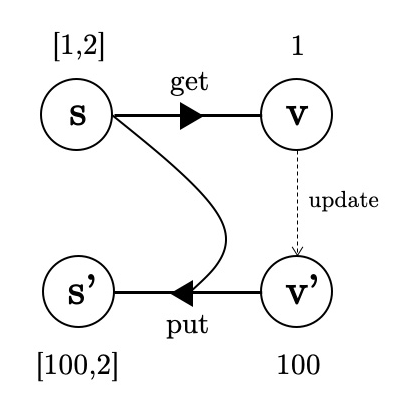
\includegraphics[height=3.5cm]{./fig/fig1.eps}
    \caption{Evaluating $phead$}
    \label{fig:eval-phead}
  \end{minipage}\hfill
  \begin{minipage}{0.7\textwidth}
    \centering
    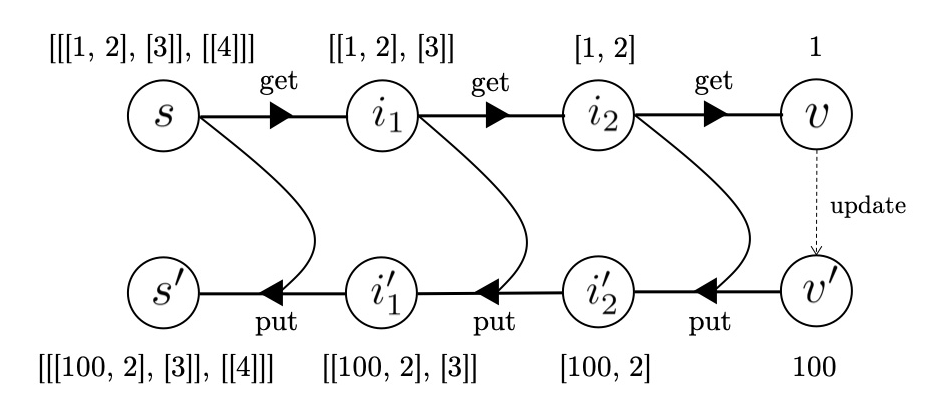
\includegraphics[height=3.5cm]{./fig/fig2.eps}
    \caption{Evaluating $phead \circ phead \circ phead$}
    \label{fig:eval-comp-phead}
  \end{minipage}
\end{figure}

Here, the original source \texttt{s}, \texttt{[1,2]}, is given by a user. $get$ is a projection: $get$ of $phead$ picks the first element of the given original source as a view.
%\texttt{get pHead [1,2] = 1}.
After the view \texttt{v} is obtained, the user can modify the view.
In this case, he or she modified the view to \texttt{100} from \texttt{1}.
From this updated view, how can we obtain new updated source? This is ``the view update problem.'' For doing this, BX provides $put$, an update function on the original source.
In this example, $put$ of $phead$ constructs a new list \texttt{[100,2]} from the updated view (\texttt{v'}) and the original source (\texttt{s}).
%\texttt{put pHead [1,2] 8 = [8,2]}

In BX programs, composition of programs is essential for writing various interesting evaluations. Because recursions are achieved by compositions, large number of programs include compositions.
In the BX lens papers \cite{} compositions are also known as central part of BX programs.
In this section we use a tiny BX program that contains compositions as a running example, because the programs including recursions can be complicated easily. The running examples are two versions of three composition of $phead$: ($phead \circ phead) \circ phead$ (we call lp3) and $phead \circ (phead \circ phead$) (we call rp3).


%For more various evaluations, we can use the composition of programs. Let us consider another example, a composition of 3 $pHead$s: $pHead \circ pHead \circ pHead$. Figure \ref{fig:eval-comp-phead} illustrates the evaluation of this program where the original source \texttt{s} is \texttt{[[[1,2],[3]],[4]]} and the updated view is \texttt{100}.
%By repetitious evaluation of $get$s of $pHead$, we can obtain the view $v$, \texttt{1}. To obtain the final updated source \texttt{s'}, we need to evaluate $put$ three times. The first put evaluation is from \texttt{i2} and \texttt{v'} and we can obtain \texttt{i2'}.

Figure \ref{fig:eval-comp-phead} illustrates the evaluation of these programs where the original source \texttt{s} is \texttt{[[[1,2],[3]],[4]]} and the updated view is \texttt{100}.
By repetitious evaluation of $get$s of $phead$, we can obtain the view $v$, \texttt{1}. To obtain the final updated source \texttt{s'}, we need to evaluate $put$ three times. The first put evaluation is from \texttt{i$_2$} and \texttt{v'} and we can obtain \texttt{i$_2$'}.

First, let us see the standard evaluation method of compositions: ``not keeping any intermediate states and obtaining them by evaluation when they are needed.'' In this example, ``intermediate states'' are \texttt{i$_1$} and \texttt{i$_2$}. This method is used in a BX language, BiGUL \cite{}. The merit of this method is clear semantics and easy to implement. The disadvantage is the number of $get$s will be quadratic when the BX programs' compositions are left associative. In the evaluation of lp3, two $get$s are required for obtaining \texttt{i$_2$} and one $get$ is required for obtaining \texttt{i$_1$}. In total, three $get$s are evaluated. We explain this method in Section 2.

If the programs are simple like these running examples, we can transform left associative compositions to right associative. However, this is not always possible. Therefore it is important to have a fast evaluation method for left associative compositions.
For achieving this, we introduce two methods that use memoization.
The first method uses memoization simply: ``keeping all intermediate states and using them when they are needed.'' There is no quadratic $get$s in this method, therefore this method improves the runtime of many BX programs. However, a disadvantage of this is the familiar tradeoff for keeping and searching values in a table. Especially, when we use large inputs, the evaluation time will be long. We explain this method in Section 3.

To treat large inputs, we introduce the second method that uses memoization: ``keeping complements in a closure and using them when they are needed.'' Complements are smaller program fragments than the original intermediate states.
%Therefore this strategy solves the previous two problems.
Readers might already know that it is a hard problem to obtain complements in general. In our work, thanks to the following finding, it is not hard:

\vspace{2mm}
In very-well behaved BX programs, 
$put$ is a complement function for $get$.
%, $get$ can be a complement function for $put$.
\vspace{2mm}

\begin{figure}[!t]
  \centering
  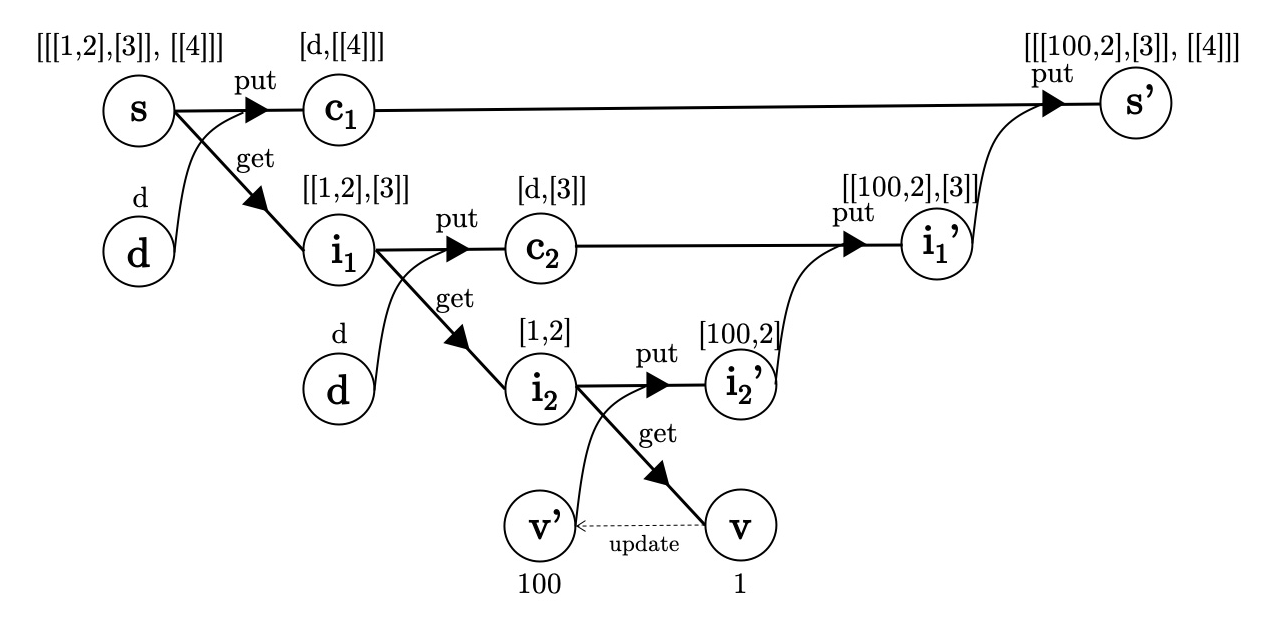
\includegraphics[height=5cm]{./fig/fig3.eps}
  \caption{Evaluating $phead \circ phead \circ phead$ by keeping intermediate states}
  \label{fig:eval-comp-phead-2}
\end{figure}

For obtaining complements, we use tupling of $put$ and $get$, and produce new function $pg$. Because $put$ produces new complements for $get$, we can shrink the size.
As an example, let us consider the previous example again: $phead \circ (phead \circ phead)$ (rp3) in figure \ref{fig:eval-comp-phead-2}. \texttt{c$_1$} and \texttt{c$_2$} are complements. The points in this figure is two. First, after evaluation of the first $pg$, we do not need to keep the original source \texttt{s}, because all its information is in \texttt{c$_1$} and \texttt{i$_1$}. Second, complements are smaller than the intermediate states in the previous figure.
%This evaluation looks better than previous two strategies: this does not require repeated evaluation and require smaller storage than the original sources. 
Actually, the simple combined $pg$ is not effective for left associative compositions, because this requires other two $put$ in the right part of the figure. To achieve efficient evaluation, we use two techniques, lazy update and lazy evaluation. We explain the second method and optimization in Section 4.

In Section 5, we show experimental results of the approaches. We discuss about related work in Section 6, and conclude in Section 7.


The contributions of this paper are the following.

\begin{itemize}
\item This is the first attempt for seriously considering efficiency of evaluation of BX compositions. Our methods are better than or similar to the results by the original method in BiGUL for all test cases.
\item We show that memoization is effective for achieving evaluation efficiency in BX languages.
\item In BX, as far as authors know optimization by $get$ and $put$ more tight is the first attempt. 
\item Although we focus on a BX language BiGUL in this paper, these techniques can be potentially used in other BX languages. 
  % \begin{itemize}
    % Although the first strategy is implemented in BiGUL \cite{}, the second and third strategies are introduced by this paper.
%  \item Thanks to introduction of the strategies, it is possible to compare the evaluation strategies.
%  \item Improvement of evaluation efficiency
%  \end{itemize}
%\item Approaches used in strategy 3
%  \begin{itemize}
%  \item 
% \item Optimization tequniques by tupling, and lazy update
%  \item These tequniques can be potentially used in other BX languages
%  \end{itemize}
\end{itemize}

